%==============================================================================
\chapter{Blockchain Fundamentals}\label{ch:bg:fundamentals}
%==============================================================================

% \begin{itemize}
% 	\item Only cover what the reader needs for the rest of the thesis. No general state of the art here.
% 	\begin{itemize}
% 		\item Check that each concept is used later on: consensus and slashing in Part III, the state model and execution in Part II, slot timing and block production in Part IV.
% 		\item Go quickly through the generic parts and spend more pages on Ethereum, since all three contributions target it.
% 	\end{itemize}
% 	\item Use Ethereum as the running example everywhere (workload in Part II, sharding in Part III, DAS in Part IV).
% 	\item Order of the chapter: ledgers, consensus, Ethereum PoS in detail, state models, execution.
% \end{itemize}

\section{Distributed Ledgers}\label{sec:bg:ledgers}

A distributed ledger is an append-only log of transactions, which is replicated by a set of nodes that do not trust each other.
Bitcoin~\cite{nakamoto2008bitcoin} was, in 2009, the first ledger of this kind to work in an open setting, and its transactions are transfers of a native currency.
In 2015, Ethereum~\cite{wood2014ethereum} extended the model so that transactions can call programs (smart contracts) whose code and storage are kept in the replicated state.
We describe here the elements of this model that are used in the rest of the thesis, and leave the question of how nodes agree on the content of the log to \autoref{sec:bg:consensus}.

\paragraph{State machine replication.}
A ledger can be seen as a case of state machine replication~\cite{schneider1990smr}.
Each node holds a copy of a state $S$ (in the simplest case, the balance of every account), and a transaction $tx$ changes it through a transition function, $S' = \delta(S, tx)$.
If all nodes start from the same initial state $S_0$, the \emph{genesis} state, and apply the same sequence of transactions $tx_1, \ldots, tx_n$, they all obtain
\[
	S_n = \delta(\ldots\delta(\delta(S_0, tx_1), tx_2)\ldots, tx_n).
\]
For this to hold, $\delta$ has to be deterministic.
The execution environments of blockchains that support smart contracts (\autoref{sec:bg:execution}) are designed with this in mind, and give programs no access to local clocks, floating-point arithmetic, or external services, all of which could give different results on different machines.
Consequently, nodes need not exchange the state to remain consistent, since it can be recomputed from the log; they only need to agree on the order of transactions, which is the role of consensus.

\paragraph{Blocks and hash chaining.}
Transactions are added to the log in batches, called blocks.
A block is made of a body, which holds the ordered list of transactions, and a header with metadata.
The header typically contains the hash of the parent header, a timestamp, and short commitments to the content of the block, such as the root of a Merkle tree over its transactions and, in some ledgers, a commitment to the state obtained after executing the block.

Because each header includes the hash of its parent, the blocks form a hash chain back to genesis.
Linking documents through hashes to detect tampering is an older idea, used for digital timestamping~\cite{haber1991timestamp}.
Under the usual assumption that the hash function is collision resistant, the hash of the most recent header fixes the whole history.
Changing a transaction in an old block changes the hash of that block, then the parent hash stored in its child, and so on up to the latest header, so a node that knows a recent header will notice the change.
Hash chaining, however, only makes a rewrite detectable.
An attacker can still produce a different, internally consistent chain, and selecting one chain among several valid candidates is again the role of consensus (\autoref{sec:bg:consensus}).

\paragraph{Merkle trees.}
These commitments are usually roots of Merkle trees~\cite{merkle1987digital}.
The leaves of a Merkle tree are hashes of data items, and every inner node is the hash of its children, so the root depends on every leaf.
A proof that an item belongs to the tree consists of the sibling hashes along the path from its leaf to the root.
Its size is logarithmic in the number of leaves, and anyone who knows the root can check it.
The same technique applies to the state.
If the header contains the root of a tree built over all state entries, such as account balances or the storage of contracts, then any single entry can be proven against that root.
How the state is organized in practice depends on the transaction and state model of the ledger, which we discuss in \autoref{sec:bg:state-model}.

\paragraph{Permissioned and permissionless ledgers.}
Ledgers also differ in who is allowed to maintain them.
In a permissioned ledger such as Hyperledger Fabric~\cite{androulaki2018hyperledger}, participants are known in advance and authenticated, and classical Byzantine fault-tolerant protocols (\autoref{sec:bg:consensus:bft}) can be used as they are, since these assume a fixed set of $n$ nodes with at most $f$ faulty ones.
Public blockchains such as Bitcoin are permissionless: anyone can join or leave, and an identity is a public key that costs nothing to generate.
A single participant can then create as many identities as it wants (a Sybil attack~\cite{douceur2002sybil}), and votes cannot simply be counted per identity.
Voting power is instead tied to a resource that is hard to obtain, computation in proof-of-work (\autoref{sec:bg:consensus:pow}) or locked stake in proof-of-stake (\autoref{sec:bg:consensus:pos}).

This thesis only considers permissionless ledgers.
For our contributions, this means that the mechanisms we add, namely the placement of state on shards in Part~III and the assignment of data to nodes in Part~IV, have to work with open membership and with some malicious participants.
These decisions must also be verifiable by any node, and resistant to bias from participants who would benefit from a particular outcome.

\paragraph{Node roles.}
Not all nodes do the same work~\cite{chatzigiannis2022sok}.
A full node checks every new block by re-executing its transactions and verifying that the result matches the commitments in the header.
It keeps the current state, and possibly a limited window of recent states.
A new full node does not usually replay the chain from genesis: it starts from a recent checkpoint, downloads the corresponding state, and validates blocks from that point on.
Under proof-of-stake, the node has to obtain this checkpoint from a source it trusts, which is related to the weak subjectivity issue discussed in \autoref{sec:bg:consensus:pos}.
An archive node is a full node that also keeps all historical states, so that it can answer queries such as the balance of an account at a given past block, at the price of a much larger disk footprint.
Validators (miners under proof-of-work) are full nodes that also propose and vote on blocks; under proof-of-stake, they are the participants that have locked stake (\autoref{sec:bg:consensus:pos}).
Finally, light clients only follow block headers and check individual values with Merkle proofs~\cite{chatzigiannis2022sok}.
They do not re-execute transactions, and instead assume that most consensus participants are honest (\autoref{sec:bg:workload:light}).

\paragraph{Peer-to-peer network.}
Nodes are connected by a peer-to-peer overlay in which each node maintains a bounded number of connections.
Transactions and blocks are propagated by gossip, where a node that receives a valid message forwards it to some of its neighbors~\cite{demers1987epidemic}.
Peers are found through a discovery protocol, often a distributed hash table such as Kademlia~\cite{maymounkov2002kademlia}.
To keep the bandwidth cost bounded, practical gossip protocols send full messages only to a small set of neighbors and announce them to the others with short metadata.

The network affects the protocol because the propagation delay of blocks bounds the rate at which blocks can be produced without degrading security~\cite{garay2015backbone,gervais2016security}.
Block intervals are therefore chosen to be large compared to this delay.
Part~IV works at this level, since its goal is to distribute and sample data over the peer-to-peer network within the time that consensus allows.

\paragraph{Full replication.}
In the model described so far, every full node stores the whole state and re-executes every transaction of every new block.
This full replication removes the need to trust other nodes, but it also implies that the capacity of the system does not increase with the number of nodes.
Throughput is limited by what a single node, run by a regular participant, can download, store, and execute.
Larger or more frequent blocks would raise this limit, but they would also increase the cost of running a node, thereby reducing the number of participants able to do so, and slow down block propagation, which results in more forks and weaker security~\cite{gervais2016security}.
\autoref{ch:bg:scalability} discusses this problem and the main approaches to it.
This thesis builds on one of them, sharding, in which each node only processes a subset of the transactions and of the data.

\section{Consensus}\label{sec:bg:consensus}

As seen in \autoref{sec:bg:ledgers}, nodes that apply the same transactions in the same order end up with the same state.
The role of the consensus protocol is to make them agree on this order, block after block, even though some of them may be faulty or malicious and messages may be delayed by the network~\cite{lamport1982byzantine}.

\paragraph{Fault and network models.}
Consensus protocols for blockchains generally assume \emph{Byzantine} faults, meaning that a faulty node may behave arbitrarily.
It can stop responding, send wrong messages, collude with other faulty nodes, or \emph{equivocate}, i.e., send conflicting messages to different nodes (e.g., votes for two different blocks at the same height).
Protocols also differ in what they assume about the network.
In the synchronous model, every message is delivered within a known bound $\Delta$.
In the asynchronous model, there is no such bound, and Fischer, Lynch, and Paterson showed that no deterministic protocol can then guarantee agreement if even one node may crash~\cite{fischer1985impossibility}.
The partially synchronous model lies in between: the network may behave asynchronously for some time, but eventually delivers messages within a bound, and agreement is possible as long as fewer than a third of the nodes are Byzantine~\cite{dwork1988partial}.
Longest-chain protocols assume a synchronous network~\cite{garay2015backbone}, whereas most BFT protocols target partial synchrony~\cite{castro1999pbft,yin2019hotstuff}.

\paragraph{Safety and liveness.}
The properties expected from consensus are usually split in two.
\emph{Safety} requires that honest nodes never confirm two conflicting blocks, so that a confirmed transaction is never reverted.
\emph{Liveness} requires that the protocol keeps making progress, so that a valid transaction submitted by an honest client is eventually included.
These two properties are in tension when the network can be partitioned.
A protocol that keeps producing blocks on both sides of a partition cannot also guarantee that these blocks will never conflict.
Some protocols therefore combine a chain that keeps growing under any conditions with a slower finality mechanism that only confirms a prefix of this chain when enough participants agree on it~\cite{neu2021ebb}.
Ethereum follows this design, as we detail in \autoref{sec:bg:eth-pos}.

\paragraph{Sybil resistance.}
Since votes in a permissionless ledger are weighted by a costly resource rather than counted per identity (\autoref{sec:bg:ledgers}), security assumptions are expressed in terms of this resource, for instance that honest participants control a majority of the computing power in proof-of-work (\autoref{sec:bg:consensus:pow}), or more than two thirds of the stake in proof-of-stake (\autoref{sec:bg:consensus:pos}).
Classical Byzantine fault-tolerant protocols (\autoref{sec:bg:consensus:bft}) do not provide Sybil resistance by themselves, but they are often run on top of proof-of-stake, by a committee selected according to stake.

\subsection{Proof-of-Work}\label{sec:bg:consensus:pow}

Proof-of-work was originally proposed to limit spam by requiring a small computation for every email~\cite{dwork1992pricing}, and Bitcoin used it to elect who appends the next block~\cite{nakamoto2008bitcoin}.
To produce a valid block, a miner has to find a value (nonce) such that the hash of the block header falls below a target.
The only known way to do so is to try values one after the other, so the probability that a given miner finds the next block is proportional to its share of the total computing power.
The target is adjusted periodically so that blocks are produced at a roughly constant rate, every ten minutes on average in Bitcoin.

Two miners may find a block at nearly the same time, in which case the chain temporarily splits into two branches, or \emph{forks}.
Nodes resolve forks with a \emph{fork-choice rule}.
Bitcoin uses the longest chain rule, or more precisely the chain with the most accumulated work, and miners extend the branch selected by this rule.
GHOST~\cite{sompolinsky2015ghost} proposed instead to follow the heaviest subtree, which also counts the blocks on discarded branches and remains secure at higher block rates.
The fork-choice rules of later proof-of-stake protocols build on this idea (\autoref{sec:bg:eth-pos:forkchoice}).

Under these rules, finality is only probabilistic.
A block can always be reverted by a heavier branch, but the probability of this decreases exponentially with the number of blocks built on top of it, which is why users wait for several confirmations.
The Bitcoin backbone analysis~\cite{garay2015backbone} shows that the protocol is secure if honest miners hold a majority of the computing power and if blocks propagate quickly compared to the block interval.
When blocks are larger or produced more often, more forks occur, and the computing power spent on discarded branches no longer contributes to security~\cite{gervais2016security}.
Throughput cannot therefore be increased simply by changing these parameters, which is the starting point of \autoref{ch:bg:scalability}.
Proof-of-work also has a high energy cost, since security is proportional to the computation spent by miners.

\subsection{Proof-of-Stake}\label{sec:bg:consensus:pos}

In proof-of-stake, participants called \emph{validators} lock an amount of currency, their \emph{stake}, and their weight in the protocol is proportional to it.
Validators are rewarded for proposing blocks and voting correctly.
Ouroboros~\cite{kiayias2017ouroboros} and Algorand~\cite{gilad2017algorand} are two examples with formal security proofs.
Ouroboros keeps a longest-chain structure and selects block producers according to stake.
Algorand selects small committees by cryptographic sortition, and each committee runs a Byzantine agreement protocol to decide on a block.

Because the stake is held by the protocol itself, misbehavior can be punished directly.
If a validator equivocates (e.g., by signing two different blocks for the same position), the two signed messages are a proof of misbehavior that identifies the culprit~\cite{sheng2021forensics}.
Anyone can include this proof in a block, and the protocol then destroys part of the validator's stake, which is called \emph{slashing}.
Security therefore rests on economic incentives, since an attack requires a large share of the stake and exposes that stake to slashing.
We come back to rewards and slashing in \autoref{sec:bg:eth-pos:safeguards}, as Part~III relies on them.

Proof-of-stake protocols need to select, at each step, the proposer of the next block and the members of the committees that vote on it.
This selection is done using randomness that is itself produced by the protocol~\cite{gilad2017algorand}.
If participants can predict this randomness long in advance, they can prepare attacks on the selected nodes, and if they can influence it, they can increase their chances of being selected for positions that benefit them.
Such manipulation has been shown to be possible in practice~\cite{nagy2025forking}.
Our designs face the same issue, since both assign tasks to nodes based on this randomness (\autoref{sec:bg:eth-pos:committees}).

Proof-of-stake also raises some issues that do not exist with proof-of-work.
Since producing a block costs almost nothing, a validator could vote on every competing branch at no cost, the so-called \emph{nothing-at-stake} problem, which slashing is designed to prevent.
Validators that have withdrawn their stake can no longer be slashed, but their old keys can still be used to sign an alternative history starting from far in the past, which is called a \emph{long-range attack}.
As a consequence, a node joining the network cannot tell the correct chain from such an alternative using only the genesis block, and has to obtain a recent checkpoint from a source it trusts.
This assumption is known as \emph{weak subjectivity}.

\subsection{BFT Variants}\label{sec:bg:consensus:bft}

Classical Byzantine fault-tolerant (BFT) protocols, starting with PBFT~\cite{castro1999pbft}, assume a fixed and known set of $n$ nodes, of which at most $f$ are Byzantine, with $n \geq 3f+1$.
Decisions are taken by \emph{quorums} of $2f+1$ nodes.
Any two such quorums share at least $f+1$ nodes, and therefore at least one honest node, which never votes for two conflicting values.
Two conflicting decisions can thus never both gather a quorum.
In PBFT, a leader proposes a value, and the nodes agree on it in three phases (pre-prepare, prepare, and commit).
If the leader is faulty or too slow, the nodes run a \emph{view change} to replace it~\cite{castro1999pbft}.
Unlike longest-chain protocols, BFT protocols give immediate finality: once a decision is taken, it is never reverted as long as the bound on $f$ holds.

The main limitation of these protocols is the number of messages they exchange.
In PBFT, every node sends its votes to every other node, so each decision requires $O(n^2)$ messages, which limits the number of participants in practice.
HotStuff~\cite{yin2019hotstuff} reduces this cost to $O(n)$ per decision by having the leader collect the votes and combine them into a single threshold signature.
Signature aggregation schemes such as BLS~\cite{boneh2001short} are used in the same way to combine thousands of votes into a single signature that can be verified at once.

Sharded blockchains such as OmniLedger~\cite{omniLedger} and RapidChain~\cite{rapidchain} run a BFT protocol inside each shard, among a committee of nodes assigned to it.
Smaller committees reach agreement faster, but they are more likely to contain more than a third of malicious members by chance.
We discuss this trade-off between committee size and security in \autoref{sec:bg:sharding}.

\section{Ethereum Proof-of-Stake}\label{sec:bg:eth-pos}

The contributions of this thesis target Ethereum, and they depend on how its consensus protocol works.
Part~III builds on its validator committees and on its penalties, and Part~IV has to fit in the timing of its slots.
We therefore describe it in more detail than the protocols of \autoref{sec:bg:consensus}.
Unless stated otherwise, the parameters given here come from the consensus specifications~\cite{ethconsensusspecs}.

Ethereum started with proof-of-work, and switched to proof-of-stake in September 2022, in an upgrade known as \emph{the Merge}.
Since then, an Ethereum node runs two separate programs.
The \emph{consensus client} runs the \emph{beacon chain}, which manages the set of validators, assigns them to committees, and decides which blocks are part of the chain and which are final~\cite{schwarzschilling2022three}.
The \emph{execution client} keeps the state and the pool of pending transactions, and executes the transactions of each block in the Ethereum Virtual Machine (\autoref{sec:bg:execution:evm}).
The two communicate through a local interface, the Engine API: the consensus client asks the execution client to build or to check the \emph{execution payload}, which is the list of transactions carried by a beacon block.
The idea of a beacon chain that coordinates a set of validators and assigns them to committees comes from earlier sharding designs, in which the beacon chain was meant to coordinate many shard chains (\autoref{sec:bg:sharding}).
The system model of Part~III follows this design.

\subsection{Validators}\label{sec:bg:eth-pos:validators}

To become a validator, a participant deposits at least 32\,ETH in a deposit contract and runs both a consensus and an execution client.
Each validator has an \emph{effective balance}, derived from its actual balance, which determines both its weight in votes and its probability of being selected as proposer or aggregator.
Until 2025, the effective balance was capped at 32\,ETH, so that large stakeholders had to run many validators.
The Pectra upgrade raised this cap to 2048\,ETH, which allows them to merge their stake into fewer validators.
The stake is, however, unevenly distributed, as staking pools and liquid staking services control a large share of it, even though it is split across many separate validators.

Validators have three kinds of duties.
They propose a block when they are selected as the proposer of a slot.
They \emph{attest} once per epoch, i.e., they sign a vote on the current head of the chain and on the latest checkpoints (\autoref{sec:bg:eth-pos:committees}).
Some of them are also selected as aggregators, and combine the attestations of their committee into a single signature.
Finally, since the Altair upgrade, a \emph{sync committee} of 512 validators, renewed every 256 epochs (about 27 hours), signs each block header so that light clients can follow the chain without tracking the whole validator set (\autoref{sec:bg:workload:light}).

Validators enter and leave the active set through queues.
The number of validators that can be activated or that can exit in each epoch is bounded by a \emph{churn limit}, which keeps the validator set from changing too quickly, and in particular prevents an attacker from gaining a large weight in a short time.
The active set is on the order of a million validators.
At this scale, a classical BFT protocol in which every validator exchanges votes with every other (\autoref{sec:bg:consensus:bft}) is impractical, and the protocol relies instead on committees and on signature aggregation, which we describe below.

\subsection{Slots and Epochs}\label{sec:bg:eth-pos:slots}

Time is divided into \emph{slots} of 12 seconds, grouped into \emph{epochs} of 32 slots, or 6.4 minutes (\autoref{fig:bg:eth-slot}).
Each slot has a single proposer, which may publish one block.
Otherwise, the slot remains empty and the protocol proceeds to the next one.

Proposers are selected at random, weighted by effective balance, using a value called the RANDAO mix.
Each proposer includes in its block a signature over the current epoch number, and this signature is mixed into the RANDAO value.
The mix obtained at the end of an epoch is used as the seed to select proposers and committees for a later epoch.
The signature of each proposer is fixed in advance, so a proposer cannot choose its contribution.
It can, however, withhold its block, in which case its contribution is skipped.
The last proposers of an epoch can use this to choose between several possible seeds, and thus bias the selection of future proposers in their favor~\cite{nagy2025forking}.
The selection is also known before the corresponding slots, which allows nodes to prepare, but also reveals to an attacker which node to target at a given time (e.g., with a denial-of-service attack).

Within a slot, the protocol follows a fixed schedule.
At the start of the slot (0\,s), the proposer publishes its block, which is then propagated through the network.
At 4\,s, the validators of the committee assigned to this slot attest to the head of the chain as they see it, or earlier if they have already received and checked the block.
At 8\,s, aggregators publish the aggregated attestations of their committee.
A validator thus has 4 seconds to receive and check a block before voting.
If the block arrives late, or cannot be checked in time, the validator votes for the previous head, and the block is likely to be left out of the chain.
In Part~IV, validators must additionally verify that the data attached to the block is available, and this verification has to fit within the same 4 seconds.

\begin{figure}[t]
	\centering
	\definecolor{slotcp}{RGB}{214,96,77}
\definecolor{slotzoom}{RGB}{67,147,195}
\definecolor{phblock}{RGB}{33,102,172}
\definecolor{phatt}{RGB}{230,145,56}
\definecolor{phagg}{RGB}{77,146,33}
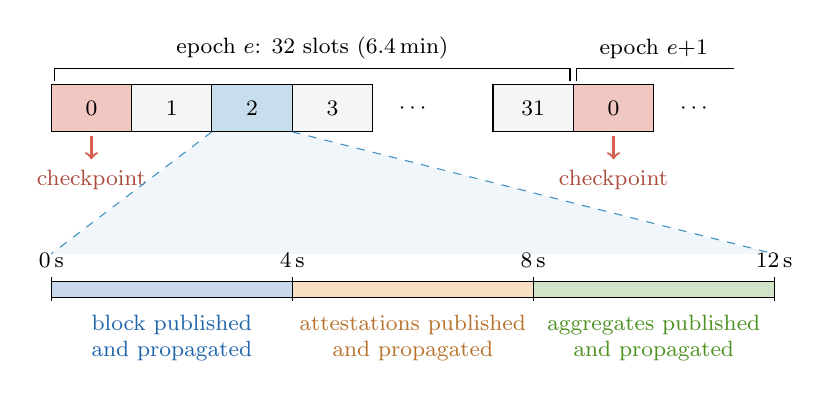
\begin{tikzpicture}[x=0.85cm,y=1cm,font=\footnotesize]
	% Zoom area, drawn first so it stays behind the labels
	\fill[slotzoom!8] (2.4,3) -- (0,1.45) -- (10.8,1.45) -- (3.6,3) -- cycle;
	% One epoch: 32 slots, a few of them drawn
	\draw[fill=slotcp!35] (0,3) rectangle ++(1.2,0.6);
	\node at (0.6,3.3) {0};
	\foreach \i/\lab in {1/1,3/3} {
		\draw[fill=gray!8] (\i*1.2,3) rectangle ++(1.2,0.6);
		\node at (\i*1.2+0.6,3.3) {\lab};
	}
	\draw[fill=slotzoom!30] (2.4,3) rectangle ++(1.2,0.6);
	\node at (3.0,3.3) {2};
	\node at (5.4,3.3) {$\cdots$};
	\draw[fill=gray!8] (6.6,3) rectangle ++(1.2,0.6);
	\node at (7.2,3.3) {31};
	\draw[fill=slotcp!35] (7.8,3) rectangle ++(1.2,0.6);
	\node at (8.4,3.3) {0};
	\node at (9.6,3.3) {$\cdots$};
	% Epoch brackets
	\draw (0.05,3.65) -- (0.05,3.8) -- (7.75,3.8) -- (7.75,3.65);
	\node[above] at (3.9,3.8) {epoch $e$: 32 slots ($6.4$\,min)};
	\draw (7.85,3.65) -- (7.85,3.8) -- (10.2,3.8);
	\node[above] at (9.0,3.8) {epoch $e{+}1$};
	% Checkpoints
	\draw[->,slotcp,thick] (0.6,2.95) -- ++(0,-0.3) node[below,text=slotcp!80!black] {checkpoint};
	\draw[->,slotcp,thick] (8.4,2.95) -- ++(0,-0.3) node[below,text=slotcp!80!black] {checkpoint};
	% Zoom on slot 2
	\draw[dashed,slotzoom] (2.4,3) -- (0,1.45);
	\draw[dashed,slotzoom] (3.6,3) -- (10.8,1.45);
	% Slot timeline, one colour per phase
	\fill[phblock!25] (0,0.9) rectangle (3.6,1.1);
	\fill[phatt!30]   (3.6,0.9) rectangle (7.2,1.1);
	\fill[phagg!25]   (7.2,0.9) rectangle (10.8,1.1);
	\draw (0,0.9) rectangle (10.8,1.1);
	\foreach \x/\t in {0/0\,s,3.6/4\,s,7.2/8\,s,10.8/12\,s} {
		\draw (\x,0.85) -- (\x,1.15);
		\node[above] at (\x,1.15) {\t};
	}
	\node[align=center,anchor=north,text=phblock] at (1.8,0.8) {block published\\and propagated};
	\node[align=center,anchor=north,text=phatt!80!black] at (5.4,0.8) {attestations published\\and propagated};
	\node[align=center,anchor=north,text=phagg] at (9.0,0.8) {aggregates published\\and propagated};
\end{tikzpicture}

	\caption{Slots and epochs in Ethereum proof-of-stake.
		An epoch has 32 slots of 12 seconds, and the first slot of each epoch serves as its checkpoint.
		Within a slot, the block is published at 0\,s, attestations at 4\,s, and aggregated attestations at 8\,s.}
	\label{fig:bg:eth-slot}
\end{figure}

\subsection{Committees and Attestations}\label{sec:bg:eth-pos:committees}

At each epoch, the active validators are shuffled using the RANDAO seed and split into committees.
Each slot of the epoch receives between 1 and 64 committees, and every validator belongs to exactly one committee in the epoch, so that it attests exactly once per epoch.
Committees have a target size of 128 validators, a size chosen so that a committee is very unlikely to have a dishonest majority as long as the attacker controls less than a third of the stake.
With around a million validators, the actual committees are much larger than this minimum.

The shuffle is deterministic and depends only on public data, i.e., the seed and the list of active validators.
Any node can therefore recompute the committees and check that a given attestation comes from a member of the right committee, without trusting anyone.
Both of our designs assign tasks to nodes in the same way, with a deterministic function of public randomness that any node can recompute.
In Part~III, it is used to elect the validator that computes the placement of state on shards, and the witnesses that check it.
In Part~IV, it determines which node is responsible for which part of the data.

An attestation contains three votes.
The \emph{head vote} designates the block that the validator considers to be the head of the chain, and is used by the LMD-GHOST fork-choice rule.
The \emph{source} and \emph{target} votes designate two checkpoints, and are used by the Casper FFG finality mechanism~\cite{schwarzschilling2022three}.
Attestations are signed with BLS signatures~\cite{boneh2001short}, which can be aggregated: the signatures of all the members of a committee who cast the same vote are combined into a single signature, together with a bit field indicating who signed.
Without aggregation, blocks would have to include about a million signatures per epoch, which would exceed the bandwidth available to nodes.

\subsection{Fork-Choice Rule}\label{sec:bg:eth-pos:forkchoice}

The consensus protocol of Ethereum, called Gasper, combines two mechanisms~\cite{schwarzschilling2022three,neu2021ebb}.
LMD-GHOST is a fork-choice rule that selects the head of the chain and allows it to grow even when many validators are offline.
Casper FFG is a finality mechanism that runs on top of this chain and finalizes some of its blocks.
Gasper follows the ebb-and-flow design of \autoref{sec:bg:consensus}, in which the chain selected by LMD-GHOST remains available and the finalized prefix guarantees safety under network partitions~\cite{neu2021ebb}.

LMD-GHOST adapts the GHOST rule (\autoref{sec:bg:consensus:pow}) to votes.
It starts from the latest justified checkpoint and, at each fork, follows the branch whose subtree has received the most weight, counting only the latest attestation of each validator (hence \emph{latest message driven}).

Casper FFG works at the level of epochs.
The checkpoint of an epoch is the block at its first slot.
When validators holding at least two thirds of the stake attest with the same source and target, the target checkpoint becomes \emph{justified}.
A justified checkpoint becomes \emph{finalized} when the checkpoint of the next epoch is justified with it as source.
In normal conditions, a block is therefore finalized after two to three epochs, or about 13 to 19 minutes.
Reverting a finalized block would require finalizing two conflicting checkpoints.
This is only possible if at least a third of the stake signs contradictory votes, and such votes can be proven and slashed (\autoref{sec:bg:eth-pos:safeguards}).

Several attacks on this fork-choice rule have been identified.
In a balancing attack, a small number of Byzantine validators release their votes at chosen times so that honest validators remain split between two branches.
In an ex-ante reorganization, an attacker withholds a block and its votes to later outweigh the next honest block~\cite{schwarzschilling2022three}.
To mitigate these attacks, the protocol now uses \emph{proposer boost}: a block received on time, before the 4\,s mark, temporarily receives additional weight in the fork choice, equal to a fraction of the weight of a committee.

Validators are expected to vote only for blocks that are valid and whose data is \emph{available}, meaning that anyone can download it.
With Data Availability Sampling, introduced in \autoref{sec:bg:l2}, validators check availability by downloading a few random samples of the data instead of all of it.
Under the \emph{tight} fork-choice rule, a validator performs this check before attesting, so that a block whose data cannot be retrieved never becomes the head, even if it is otherwise valid.
Under the \emph{trailing} fork-choice rule, the check is performed later, which gives more time but weaker guarantees, since a block may be built upon before its data has been checked.
Part~IV targets the tight fork-choice rule, which is why sampling has to be done within the first 4 seconds of the slot~\cite{pigaglio2025pandas}.

\subsection{Rewards and Safeguards}\label{sec:bg:eth-pos:safeguards}

Validators are paid for performing their duties correctly and on time, and lose a small amount when they miss them.
The reward for an attestation depends on whether each of its three votes is correct and on how quickly it was included in a block.
Proposers are rewarded for including attestations and evidence of misbehavior in their blocks, and members of the sync committee for signing headers.

A validator is \emph{slashed} when it signs messages that contradict each other.
There are three such cases: proposing two different blocks for the same slot, casting two attestations with the same target epoch but different content, and casting an attestation whose source and target surround those of another of its attestations~\cite{schwarzschilling2022three}.
In each case, the proposer that includes the resulting proof (\autoref{sec:bg:consensus:pos}) receives a small reward.
A slashed validator immediately loses a small part of its balance, is forced to exit, and can only withdraw its remaining funds after about 36 days.
In the middle of this period, it pays an additional \emph{correlation penalty}, which is proportional to the total stake slashed in the same time window.
An isolated fault, typically caused by a misconfiguration, therefore incurs a small penalty, whereas a coordinated attack involving a third of the stake leads to the loss of the entire stake of the attackers.

A different safeguard handles the case where finality stops.
If more than a third of the stake is offline, no checkpoint can gather two thirds of the votes, and the chain stops finalizing.
After a few epochs without finality, the \emph{inactivity leak} starts: the balances of the validators that do not participate decrease, faster and faster, until the remaining active validators again hold two thirds of the stake and finality resumes.
These penalties must, however, be designed carefully: Pavloff et al.\ show that Byzantine validators can exploit them to reduce the stake of honest validators and increase their own relative weight~\cite{pavloff2024byzantine}.

Ethereum thus does not prevent misbehavior, and instead penalizes it when it can be proven and attributed to a validator.
SOAPS (Part~III) relies on the same mechanisms (election, stake, and slashing) instead of a separate consensus protocol.
For this reason, any deviation from the SOAPS protocol must be detectable and attributable to a specific validator, and its challenge mechanism serves this purpose.

Finally, the block of each slot is not always built by its proposer.
The order of transactions in a block can be a source of profit (e.g., by placing one's own transaction just before or after a large trade), and this profit is called \emph{maximal extractable value} (MEV)~\cite{daian2020flashboys}.
Extracting MEV requires specialized infrastructure, and Ethereum has therefore adopted, outside of the protocol, a form of \emph{proposer-builder separation} (PBS).
Specialized \emph{builders} assemble blocks and bid for the right to have them proposed, and \emph{relays} forward the highest bid to the proposer, which signs the block header without seeing its content.
A small number of builders produce most of the blocks~\cite{heimbach2023pbs}.
As a result, the data distributed and sampled in Part~IV initially comes from a few well-connected and well-provisioned builders, whereas most of the nodes that sample it run on modest hardware.

\section{Transaction and State Models}\label{sec:bg:state-model}

The state machine view of \autoref{sec:bg:ledgers} leaves open what the state is made of and how a transaction designates the part of the state it reads and modifies.
The state model defines which data a transaction accesses, and therefore when two transactions conflict.
It determines whether transactions can be executed in parallel (\autoref{sec:bg:workload:parallel}) and how the state can be divided between shards (\autoref{sec:bg:sharding:state}).
The \emph{unspent transaction output} (UTXO) model, introduced by Bitcoin~\cite{nakamoto2008bitcoin}, represents the state as a set of coins, while the \emph{account-based} model, used by Ethereum~\cite{wood2014ethereum}, represents it as a set of accounts with balances and storage.
This thesis works with the account-based model, but we first describe the UTXO model, as the comparison explains several of the difficulties addressed in Parts~II and~III.

\subsection{UTXO Model}\label{sec:bg:state-model:utxo}

In the UTXO model, the state is the set of transaction outputs that have not been spent yet.
Each output holds an amount and a condition that must be satisfied to spend it, usually a signature from the owner's key.
A transaction consumes one or more existing outputs, its \emph{inputs}, and creates new ones.
Each input refers explicitly to the output it spends, by the identifier of the transaction that created it and its position in that transaction, and provides the data that satisfies its spending condition.
The total amount of the new outputs cannot exceed that of the inputs, and the difference is paid as a fee to the block producer (\autoref{fig:bg:utxo}).
An output can only be spent once.
Two transactions that spend the same output are a \emph{double spend}, and at most one of them can be included in the ledger.

\begin{figure}[t]
	\centering
	\definecolor{utxospent}{RGB}{214,96,77}
\definecolor{utxonew}{RGB}{77,146,33}
\definecolor{utxotx}{RGB}{67,147,195}
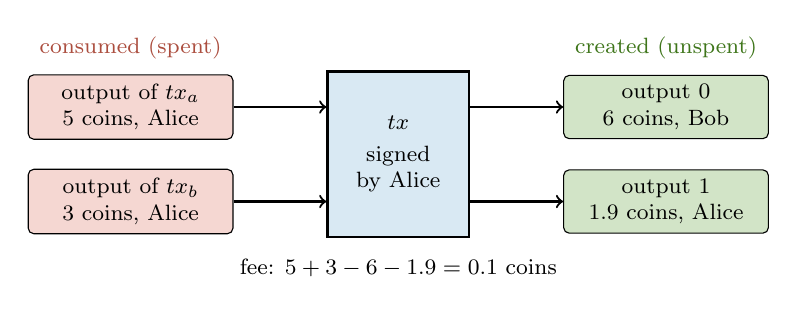
\begin{tikzpicture}[x=1cm,y=1cm,font=\footnotesize,
	utxobox/.style={draw,rounded corners=2pt,minimum width=2.6cm,minimum height=0.75cm,align=center},
	txbox/.style={draw,thick,fill=utxotx!20,minimum width=1.8cm,minimum height=2.1cm,align=center}]
	\node[utxobox,fill=utxospent!25] (i1) at (0,0.6) {output of $tx_a$\\5 coins, Alice};
	\node[utxobox,fill=utxospent!25] (i2) at (0,-0.6) {output of $tx_b$\\3 coins, Alice};
	\node[txbox] (t) at (3.4,0) {$tx$\\[2pt]signed\\by Alice};
	\node[utxobox,fill=utxonew!25] (o1) at (6.8,0.6) {output 0\\6 coins, Bob};
	\node[utxobox,fill=utxonew!25] (o2) at (6.8,-0.6) {output 1\\1.9 coins, Alice};
	\draw[->,thick] (i1.east) -- (t.west |- i1.east);
	\draw[->,thick] (i2.east) -- (t.west |- i2.east);
	\draw[->,thick] (t.east |- o1.west) -- (o1.west);
	\draw[->,thick] (t.east |- o2.west) -- (o2.west);
	\node[text=utxospent!80!black] at (0,1.35) {consumed (spent)};
	\node[text=utxonew!80!black] at (6.8,1.35) {created (unspent)};
	\node at (3.4,-1.45) {fee: $5 + 3 - 6 - 1.9 = 0.1$ coins};
\end{tikzpicture}

	\caption{A transaction in the UTXO model.
		It consumes two outputs owned by Alice, which are removed from the set of unspent outputs, and creates two new ones: a payment to Bob and the change returned to Alice.
		The difference between inputs and outputs is the fee.}
	\label{fig:bg:utxo}
\end{figure}

Since inputs are listed in the transaction, the part of the state a transaction depends on is known before it is executed.
Two transactions conflict only if they spend the same output, or if one spends an output created by the other.
Transactions that do not share outputs can be validated in parallel, and a sharded design can place each output on a shard (e.g., according to the identifier of the transaction that created it) and know in advance which shards a transaction involves.
For the same reason, several of the first sharded blockchains were designed for the UTXO model~\cite{omniLedger,rapidchain}, and transaction placement methods have been proposed for it~\cite{Nguyen2019}.

The limitation of this model is that outputs are consumed as a whole and do not hold any persistent data.
Applications that maintain shared, long-lived state, such as a token or an exchange used by many users, are therefore difficult to express.
Extended UTXO models add data and more expressive scripts to outputs while keeping explicit inputs, but they require the application to split its state into outputs that are consumed and recreated at every update.
Since the workloads we study and the systems we target use accounts, we do not consider the UTXO model further.

\subsection{Account-Based Model}\label{sec:bg:state-model:account}

In the account-based model, the state is a mapping from addresses to accounts.
In Ethereum, there are two types of accounts.
\emph{Externally owned accounts} (EOA) are controlled by a private key, and hold a balance and a \emph{nonce}, which counts the transactions sent by the account.
Each transaction carries the nonce of its sender, which forces the transactions of an account to be executed in order and prevents the same signed transaction from being replayed.
\emph{Smart contract accounts} (SCA) are created by deploying code.
In addition to a balance and a nonce, they hold this code and a persistent \emph{storage}, a mapping from 256-bit keys, called slots, to 256-bit values, which only the contract's code can modify (\autoref{sec:bg:execution}).
A token contract, for instance, typically keeps the balance of each of its holders in a separate storage slot.

A transaction is sent by an EOA.
It either transfers currency to another account, deploys a new contract, or calls an existing contract with some input data.
The called contract may in turn call other contracts, which may call others, so that a single transaction can read and modify many accounts and storage slots.
The block only contains the original transaction, and the resulting \emph{internal transactions} can only be observed by executing it (\autoref{sec:bg:execution:evm})~\cite{pigaglio2023exploring}.
Interactions are also very unevenly distributed, as a small number of accounts, such as exchanges, popular token contracts, and decentralized finance protocols, are involved in a large share of all transactions~\cite{guo2019graph}.

The main difference with the UTXO model is that the state accessed by a transaction is not known in advance.
It depends on the code of the contracts involved and on the current values in their storage, which may change between the moment the transaction is signed and the moment it is executed.
The same call can thus access different slots, or different contracts, depending on the transactions executed before it.
As a consequence, whether two transactions conflict, meaning that one writes data that the other reads or writes, is in general only known after they have been executed.
Ethereum lets a transaction declare an \emph{access list} of the accounts and slots it intends to use, but the list is optional, and the transaction can still access state that it does not list.
Parallel execution (\autoref{sec:bg:workload:parallel}) and state sharding (\autoref{sec:bg:sharding:state}) are therefore harder with accounts than with UTXOs.
Part~II measures how the accesses of real transactions are distributed over time and across transactions, and the same uncertainty complicates the placement of accounts on shards in Part~III.

Executing a transaction also has a cost, measured in \emph{gas}.
Each operation of the execution environment has a fixed gas cost, which reflects the resources it uses, and accessing or writing storage is among the most expensive operations.
The sender sets a maximum amount of gas for its transaction, and pays for the gas actually used.
Since the London upgrade, the price of gas has two components~\cite{roughgarden2021tfm}.
A \emph{base fee}, set by the protocol, increases when blocks are fuller than a target and decreases when they are emptier, and is burned.
A \emph{priority fee}, chosen by the sender, goes to the block proposer and determines which transactions it includes first when demand is high, and therefore how long a transaction waits before being included~\cite{pacheco2023my}.
Each block also has a \emph{gas limit}, which bounds the total amount of computation it may contain.
In effect, the gas limit sets the throughput of the chain.
It is kept low enough for nodes with modest hardware to execute each block within a slot, as a consequence of the full replication discussed in \autoref{sec:bg:ledgers}.

\section{Smart Contracts and Execution Environments}\label{sec:bg:execution}

A \emph{smart contract} is a program stored in the ledger, whose code is executed by every full node whenever a transaction calls it.
Its state, such as balances or open positions, is part of the replicated state, and can only be modified by the contract's own code.
Since all nodes execute the same code on the same state, a contract call produces the same result on every node, and no party needs to be trusted to execute it correctly.

A large part of the activity on Ethereum involves a few types of contracts.
Token contracts keep track of who owns which units of a fungible asset, following the ERC-20 interface, or of non-fungible items, following ERC-721.
Decentralized exchanges let users swap one token for another against pools of liquidity held by a contract.
Lending protocols let users borrow tokens against collateral, and bridges lock assets on one chain to release equivalent assets on another.
In the workload we analyze in Part~II, transactions involving smart contracts have become dominant over time, whereas simple transfers, which represented more than 80\% of early transactions, have become marginal~\cite{pigaglio2023exploring}.

Contracts can call each other, and applications are often built by composing existing contracts.
A swap on a decentralized exchange, for instance, may go through a router contract, then through one or several pools, each of which calls the token contracts of the assets it holds, so that a single transaction can involve tens of contracts.
\autoref{fig:bg:calltree} shows a simplified example, in which a two-step swap already involves six contracts.

\begin{figure}[t]
	\centering
	\resizebox{\linewidth}{!}{\definecolor{ctblock}{RGB}{33,102,172}
\definecolor{ctcall}{RGB}{230,145,56}
\definecolor{ctstate}{RGB}{77,146,33}
\begin{tikzpicture}[x=1cm,y=1cm,font=\footnotesize,
	acc/.style={draw,rounded corners=2pt,minimum height=0.6cm,inner sep=3pt,anchor=west},
	eoa/.style={acc,fill=ctblock!20},
	ctr/.style={acc,fill=gray!10},
	slots/.style={anchor=west,text=ctstate!80!black},
	call/.style={->,thick,ctcall},
	lbl/.style={font=\scriptsize\ttfamily,text=ctcall!80!black,above,pos=0.78}]
	% Transaction recorded in the block
	\node[eoa] (alice) at (0,0) {Alice (EOA)};
	\node[ctr] (router) at (2.7,0) {Router};
	\draw[->,thick,ctblock] (alice) -- node[above,font=\scriptsize,text=ctblock] {tx} (router);
	% Internal transactions
	\node[ctr] (tx) at (5.0,-1.0) {Token X};
	\node[ctr] (pa) at (5.0,-2.0) {Pool A};
	\node[ctr] (ty) at (7.0,-3.0) {Token Y};
	\node[ctr] (pb) at (5.0,-4.0) {Pool B};
	\node[ctr] (tz) at (7.0,-5.0) {Token Z};
	\coordinate (rs) at ([xshift=0.3cm]router.south west);
	\coordinate (as) at ([xshift=0.3cm]pa.south west);
	\coordinate (bs) at ([xshift=0.3cm]pb.south west);
	\draw[call] (rs) |- node[lbl] {transferFrom} (tx.west);
	\draw[call] (rs) |- node[lbl] {swap} (pa.west);
	\draw[call] (rs) |- node[lbl] {swap} (pb.west);
	\draw[call] (as) |- node[lbl] {transfer} (ty.west);
	\draw[call] (bs) |- node[lbl] {transfer} (tz.west);
	% Storage slots read and written
	\node[anchor=west,text=ctstate!80!black,font=\footnotesize\itshape] at (8.7,0) {storage slots accessed};
	\node[slots] at (8.7,-1.0) {W: bal[Alice], bal[Pool A], allowance};
	\node[slots] at (8.7,-2.0) {R/W: reserves of Pool A};
	\node[slots] at (8.7,-3.0) {W: bal[Pool A], bal[Pool B]};
	\node[slots] at (8.7,-4.0) {R/W: reserves of Pool B};
	\node[slots] at (8.7,-5.0) {W: bal[Pool B], bal[Alice]};
	\foreach \n/\y in {tx/-1,pa/-2,pb/-4} \draw[densely dotted,gray] (\n.east) -- (8.65,\y);
	\foreach \n/\y in {ty/-3,tz/-5} \draw[densely dotted,gray] (\n.east) -- (8.65,\y);
	% Brackets on the left
	\draw[ctblock,thick] (-0.15,0.35) -- (-0.3,0.35) -- (-0.3,-0.35) -- (-0.15,-0.35);
	\node[anchor=east,align=right,text=ctblock] at (-0.35,0) {in the\\block};
	\draw[ctcall,thick] (-0.15,-0.7) -- (-0.3,-0.7) -- (-0.3,-5.3) -- (-0.15,-5.3);
	\node[anchor=east,align=right,text=ctcall!80!black] at (-0.35,-3.0) {internal\\trans-\\actions,\\only in\\the trace};
\end{tikzpicture}
}
	\caption{Calls made by a transaction in which Alice swaps token X for token Z through two exchange pools (X to Y in Pool A, then Y to Z in Pool B).
		Only the transaction from Alice to the router is recorded in the block.
		The internal transactions, and the storage slots that each contract reads (R) and writes (W), are only visible by executing the transaction.}
	\label{fig:bg:calltree}
\end{figure}

These calls create the dependencies between accounts in the account-based model (\autoref{sec:bg:state-model:account}).
They also explain why some contracts, such as widely used tokens or exchange pools, are accessed by a large fraction of all transactions, and become contention points when transactions are executed in parallel or when the state is split between shards.

\subsection{The Ethereum Virtual Machine}\label{sec:bg:execution:evm}

Ethereum contracts are executed by the Ethereum Virtual Machine (EVM)~\cite{wood2014ethereum}.
The EVM is a stack machine that operates on 256-bit words.
During a call, a contract has access to a stack, a temporary \emph{memory} that is discarded at the end of the call, the input data of the call, and its persistent \emph{storage} (\autoref{sec:bg:state-model:account}).
Each instruction has a gas cost, and execution stops with an error when the gas provided by the transaction runs out, so that every execution is guaranteed to terminate.
Storage accesses are by far the most expensive instructions.
Reading a storage slot for the first time in a transaction costs hundreds of times more gas than an arithmetic operation, and writing a slot that was previously zero costs even more, because these operations require accessing and updating the state database of every node.

A contract calls another contract with the \texttt{CALL} instruction, which runs the code of the callee on the callee's storage.
\texttt{STATICCALL} does the same but forbids any modification of the state, and \texttt{DELEGATECALL} runs the code of the callee on the storage of the caller, which is how libraries and upgradable contracts are implemented.
If a call fails, its changes to the state are reverted, but the caller can continue and decide how to handle the failure.
Transactions in a block are executed one after the other, in the order chosen by the block producer, and each transaction sees the state left by the previous one.

The state is stored in Merkle Patricia Tries, which combine the Merkle trees of \autoref{sec:bg:ledgers} with a prefix tree (Patricia trie), so that each key determines a unique path from the root to its value.
The state is organized in two levels.
The \emph{world-state trie} maps the hash of each address to the corresponding account, which contains its nonce, balance, code hash, and storage root.
Each contract has its own \emph{storage trie}, which maps the hash of each storage slot to its value.
The root of the world-state trie is the state root included in each block header.
Reading a value requires following a path from the root of the trie down to a leaf, which can take several disk accesses.
Since keys are hashed, entries that are related in the application, such as two slots of the same contract, end up in unrelated parts of the trie and on disk.
Accessing the state is therefore one of the main costs of executing a block, and clients rely on caches and on flat copies of the latest state to reduce it.
Such caches are only effective if transactions tend to access state that was accessed recently, which is the temporal locality we measure in Part~II.

The read and write sets of a transaction cannot be obtained from the block alone, since internal transactions are not recorded in it (\autoref{sec:bg:state-model:account}).
To obtain them, we replay the whole chain with the Go Ethereum (geth) client and record, for each transaction, the accounts it reads and writes, including those accessed by its internal transactions (\autoref{fig:bg:calltree}).
Replaying the chain up to the Merge takes about three days and produces a dataset of about 2\,TB, and Part~II describes the tool we built to process it~\cite{pigaglio2023exploring}.

Sequential execution over a single global state, combined with the block gas limit that keeps execution within reach of modest nodes (\autoref{sec:bg:state-model:account}), caps Ethereum's throughput to roughly 15 to 30\,tx/s.

\subsection{Alternative Execution Environments}\label{sec:bg:execution:alternatives}

Many other blockchains, as well as most layer-2 protocols (\autoref{sec:bg:l2}), reuse the EVM.
Being EVM-compatible allows them to run existing contracts and to reuse the same development tools, and their workloads tend to resemble that of Ethereum, since they host the same kinds of applications.
Other chains use different virtual machines (e.g., based on WebAssembly) but keep the same model of contracts executed sequentially over shared state.

A different line of work changes the execution model to allow parallel execution.
Dickerson et al.\ proposed that block producers execute contract calls speculatively in parallel, and publish the resulting schedule so that validators can replay the block in parallel and deterministically~\cite{dickerson2017concurrency}.
Several recent blockchains were designed with parallel execution in mind.
In Solana, each transaction declares the accounts it will read and write, and the runtime executes in parallel the transactions whose accounts do not overlap.
Sui represents the state as objects, and distinguishes objects owned by a single user from shared objects.
Transactions that only use owned objects do not need to be ordered with respect to others and can bypass consensus, and only transactions on shared objects go through consensus~\cite{blackshear2024sui}.
Aptos uses Block-STM, which executes the transactions of a block optimistically in parallel, detects conflicts at runtime, and re-executes the transactions involved, so that the result is the same as a sequential execution in the order of the block~\cite{gelashvili2023blockstm}.

These designs follow two approaches.
Either transactions declare their dependencies in advance, which is easy in the UTXO model but constrains how contracts are written in the account-based model, or the system executes optimistically and assumes that conflicts are rare.
In both cases, the benefit depends on the workload: transactions that access the same accounts must still be executed sequentially.
\autoref{sec:bg:workload} discusses these techniques further, and Part~II measures to what extent real transactions allow them.
